\chapter{Title of Chapter Five}
\label{chap:five}

\section{Frequently made mistakes}

The following checklist should help in avoiding some frequently made mistakes, if any of the following propositions apply for your thesis, there is a problem:

\begin{itemize} 
		\item You have citations in your abstract.
		\item The introduction does not cover the three parts as described in \autoref{chap:one}.
		\item The introduction contains subheadings.
		\item You described different aspects than promised in the title.
		\item You copied some parts of the text from other work without proper referencing and citing.
		\item You used automatic translation tools to produce text by translating it from another language.
		\item Your thesis contains many typos and grammatical errors. (Use an electronic spell checker. Please!)
		\item You used color in your figures and refer to the ``blue'' line (assume that your readers use a monochrome printer).
		\item You mainly used websites and other unrefereed material as your sources or you used Wikipedia as your source.
		\item You refer to something in your conclusion which you have not mentioned before.
		\item Some forenames in the references are abbreviated, some not.
		\item Some references miss a publishing date.
\end{itemize}


\section{Useful Hints}

If you write in English, you might find the following hint
useful: The indefinite article a is used as an before a
vowel sound---for example an apple, an hour, an unusual
thing, an \ac{MNC} (because the acronym is pronounced Em-En-See). Before a consonant sound represented
by a vowel letter a is usual---for example a one, a
unique thing, a historic chance. Few more tips to follow:


\begin{itemize}
\item Don't give orders---don't write in the imperative mood---unless you are training to be a teacher.
\item Avoid the use of questions. You may know the answer: does your reader?
It's much safer to tell her, or him.
\item Do not become entangled in the problems of `sexist' language.
It is much easier to write in the plural.
``Students should check their work'' is good English.
``A student should check---'' is also good English, but now the problems begin: ``---her work?'' ``---his work?''
Which? You can write ``his or her,'' but that seems clumsy. Stick to the plural.
\item If you must refer to yourself, use the third person such as ``The present writer would recommend that \ldots'' may be useful.
\item Use the full forms of words and phrases, not contractions like ``he's,'' ``don't,'' etc.
Keep the apostrophe to indicate possession---and use it correctly.
Academics really sneer at students who use the ``Greengrocer's apostrophe.''
\end{itemize}


\begin{itemize}
\item Do not despise short, workmanlike, and effective plain English words.
If they mean what you want to say. Accurately.
\item Avoid the use of humor in academic writing---unless you are very sure of yourself.
\item Even when you are not being funny, avoid the use of irony or sarcasm.
\item Paragraphs in academic English should contain more than one sentence.
(Short paragraphs look as if you are writing for a tabloid newspaper---or a simple Template!)
I guess that the average academic book runs to two or three paragraphs per page.
Look at the books in your subject, and get a feel for how long your own paragraphs should be when you are imitating the academic style.
\item Develop an academic vocabulary.
The `long words' you learn in the course of your studies are long usually because they have more precise meanings than their less formal equivalents.
They are therefore better when you want to be accurate.
(Also they allow you to sound like someone who deserves a degree.)
\end{itemize}



\begin{itemize}
\item  Use as few words as you can; but use enough words to express your meaning as fully as you can. Your judgment of what is appropriate here is part of what you should learn throughout your course.
\item  Avoid lazy words such as ``nice''.
It is usually better to say ``acquire'' or ``obtain'' than ``get;'' and it may be better, if you mean ``through the use of money,'' to say ``purchase'' or---better still---``buy.''
\item A short word like ``buy'' is better than a long one like ``purchase''---unless the long one is more accurate.
A ``statutory instrument'' is better than a ``rule''---to a lawyer, at any rate.
\item Proof-read with care.
Ask someone else to help---you may be too close to your work to be able to see your mistakes.
\item If in doubt, choose the more formal, or possibly just the more old-fashioned, of two words.
For example, say quotation rather than quote whenever you mean the use of somebody else's words.
\end{itemize}



\begin{itemize}
\item You will often sound more academic if you include doubts in your work---and qualifications.
Within the scope of this thesis, the current writer cannot hope to cover all the possible implications of the question.
\item In this context, the use of litotes sounds very academic.
This is the construction where a writer uses a negative with a negative adjective, e.g.\ it is not unlikely that \ldots This does not mean the same as it is probable that \ldots It has a shade of meaning and qualification that can be useful to academic writers.
\end{itemize}


Text text  \citet{Haufler2006}.

Text text text text text text text \cite[see, \latinfont{inter alia},][pg.~10]{Haaparanta1996}. 

Special Czech, Slovak, and German letters:

\r{u}, \'{a}, \v{s}, \v{d}, \v{t}, \v{r}, \^{o}, \ss{}, \"{o}


\section{Itemization and Environments}

Many people use simple n-dash in many occasions -- like this --, where however typographic convention---it looks a bit strange at first sight---requires m-dash.
Text text text text text text \citet{Haufler2006}. 

Text text text text text text \citet{Wells2001}. Let us describe the following animals:

\begin{description}
\item[Item 1] Text.
\item[Item 2] Text.
\end{description}

See what Edmund Burke said about the duties of a Member of Parliament (Speech To The Electors Of Bristol At The Conclusion Of The Poll, November 3, 1774):

\begin{quotesmall}
It ought to be the happiness and glory of a representative to live in the strictest union, the closest correspondence, and the most unreserved communication with his constituents. 
Their wishes ought to have great weight with him; their opinion, high respect; their business, unremitted attention.
It is his duty to sacrifice his repose, his pleasures, his satisfactions, to theirs; and above all, ever, and in all cases, to prefer their interest to his own.
But his unbiased opinion, his mature judgment, his enlightened conscience, he ought not to sacrifice to you, to any man, or to any set of men living.
These he does not derive from your pleasure; no, nor from the law and the constitution.
They are a trust from Providence, for the abuse of which he is deeply answerable.
Your representative owes you, not his industry only, but his judgment; and he betrays, instead of serving you, if he sacrifices it to your opinion.
\end{quotesmall}

Text text text text.

\begin{listi}
	\item The first item, the first item, the first item, the first item, the first item, the first item,
	\item and the second item.
\end{listi}

\begin{lista}
	\item The first item, the first item, the first item, the first item, the first item, the first item, 
	\item and the second item.
\end{lista}

TText text text text text text \citet{Blomstrom2003}. 

\section{Acronyms}

Politicians usualy like inward \ac{FDI} and an \ac{MNC} appreciates \ac{FDI} subsidies. Are \acp{MNC} greedy?

\section{Figures}

To achieve compatibility with PDF/A 2u, your file must not include links to external fonts, audio, video, or scripts. On the other hand, your file must declare each color environment you use, it must include all the pictures/figures either in jpeg or PDF/A 2u format, used fonts compliant under Unicode (your file cannot use any external fonts), and it must include meta-data in XMP format.


Most troubleshooting comes from the conversion of figures to compliant formats. You can convert from simple PDF using Adobe Acrobat:
\begin{itemize}
	\item Select File >> Save as Other >> Archivable PDF (PDF/A)
				\begin{figure}[!h]
					\centering
						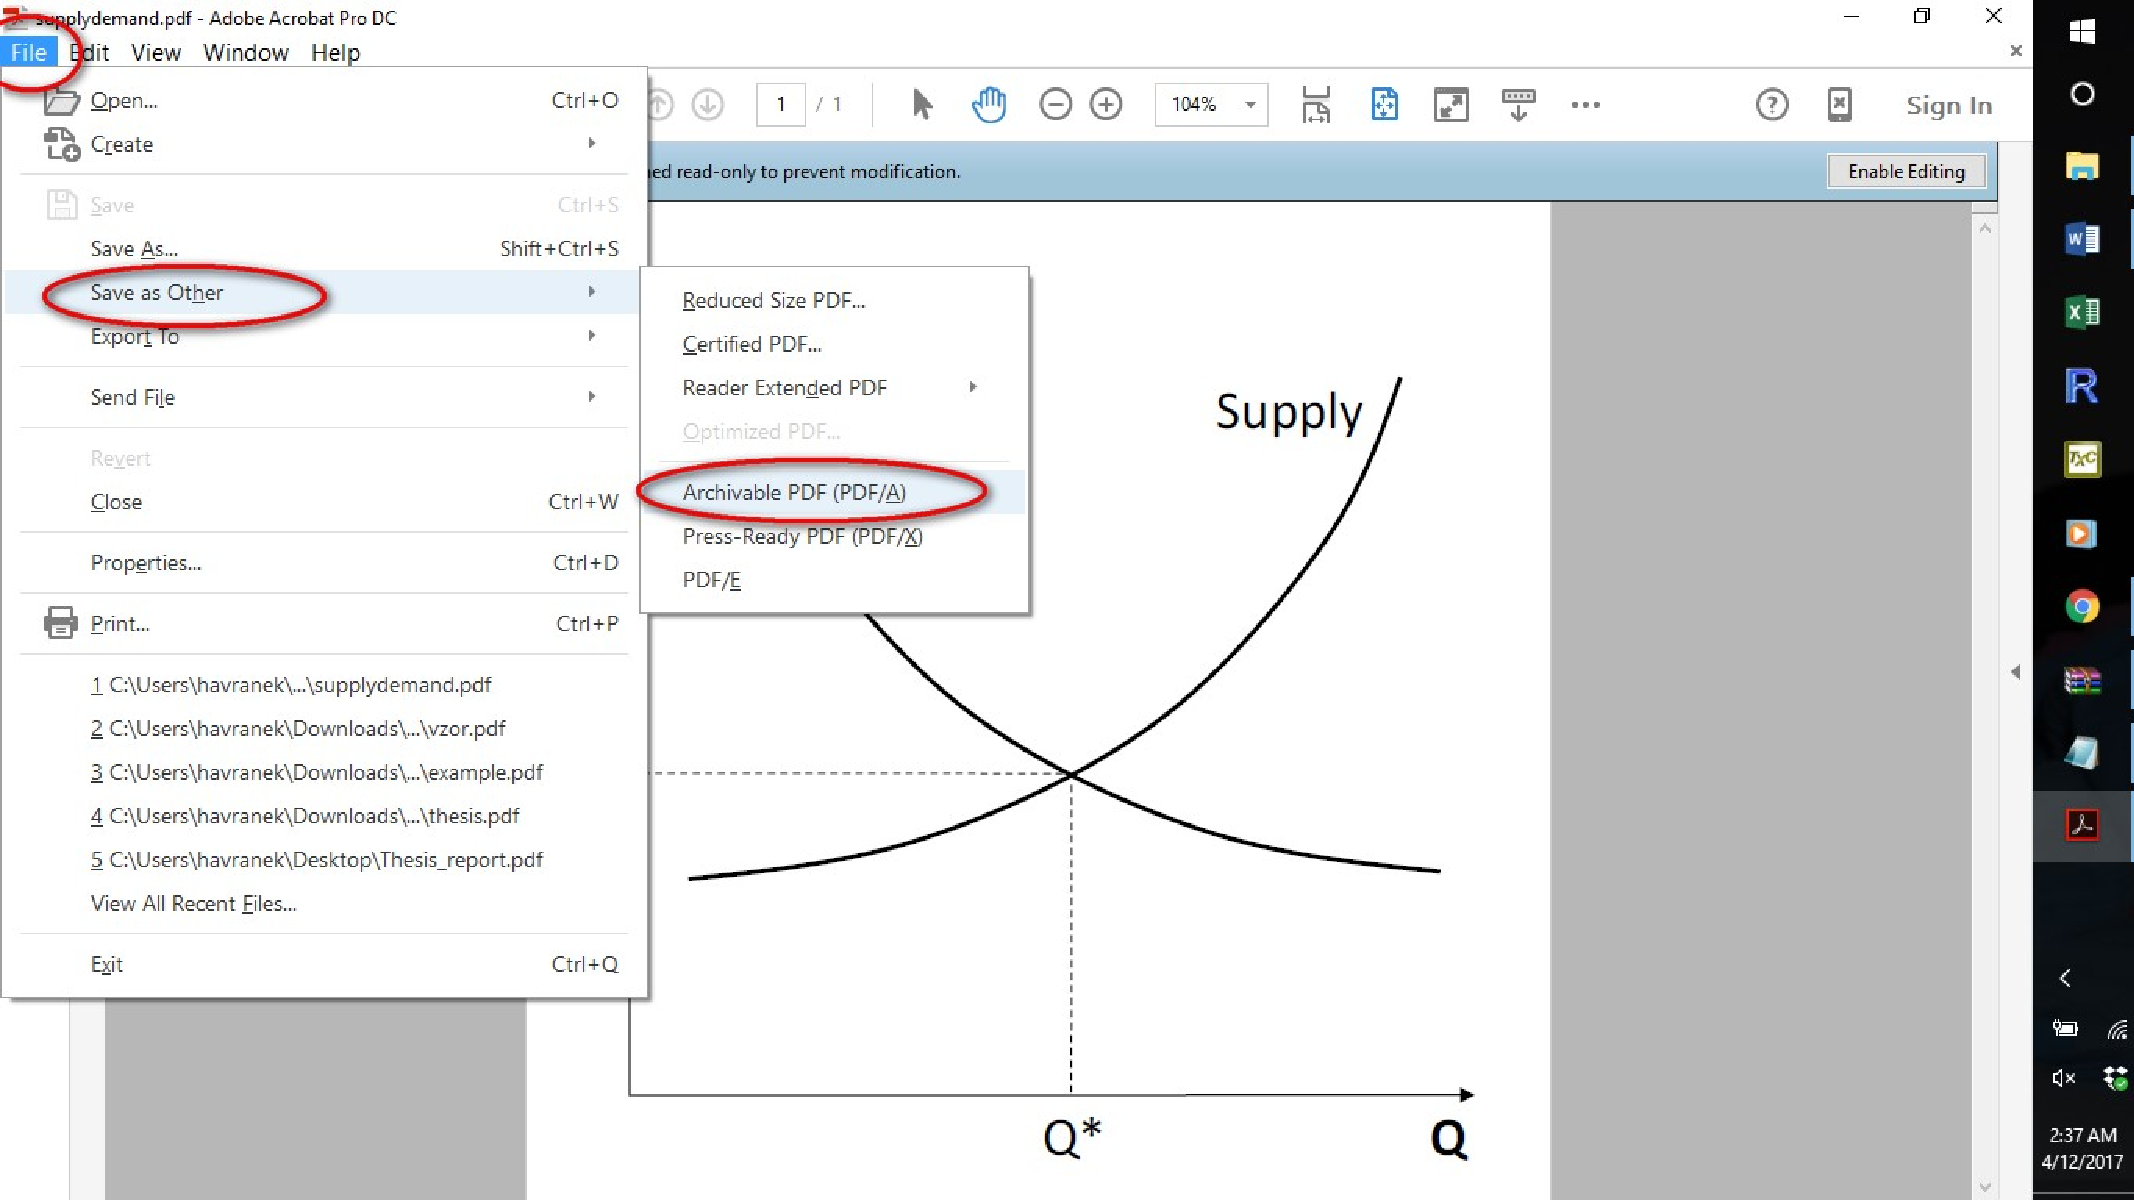
\includegraphics[width=0.6\textwidth]{Figures/conversion1.pdf}
					\label{fig:conversion1}
				\end{figure}
	\item Save as PDF/A-2u:
			\begin{figure}[!h]
				\centering
					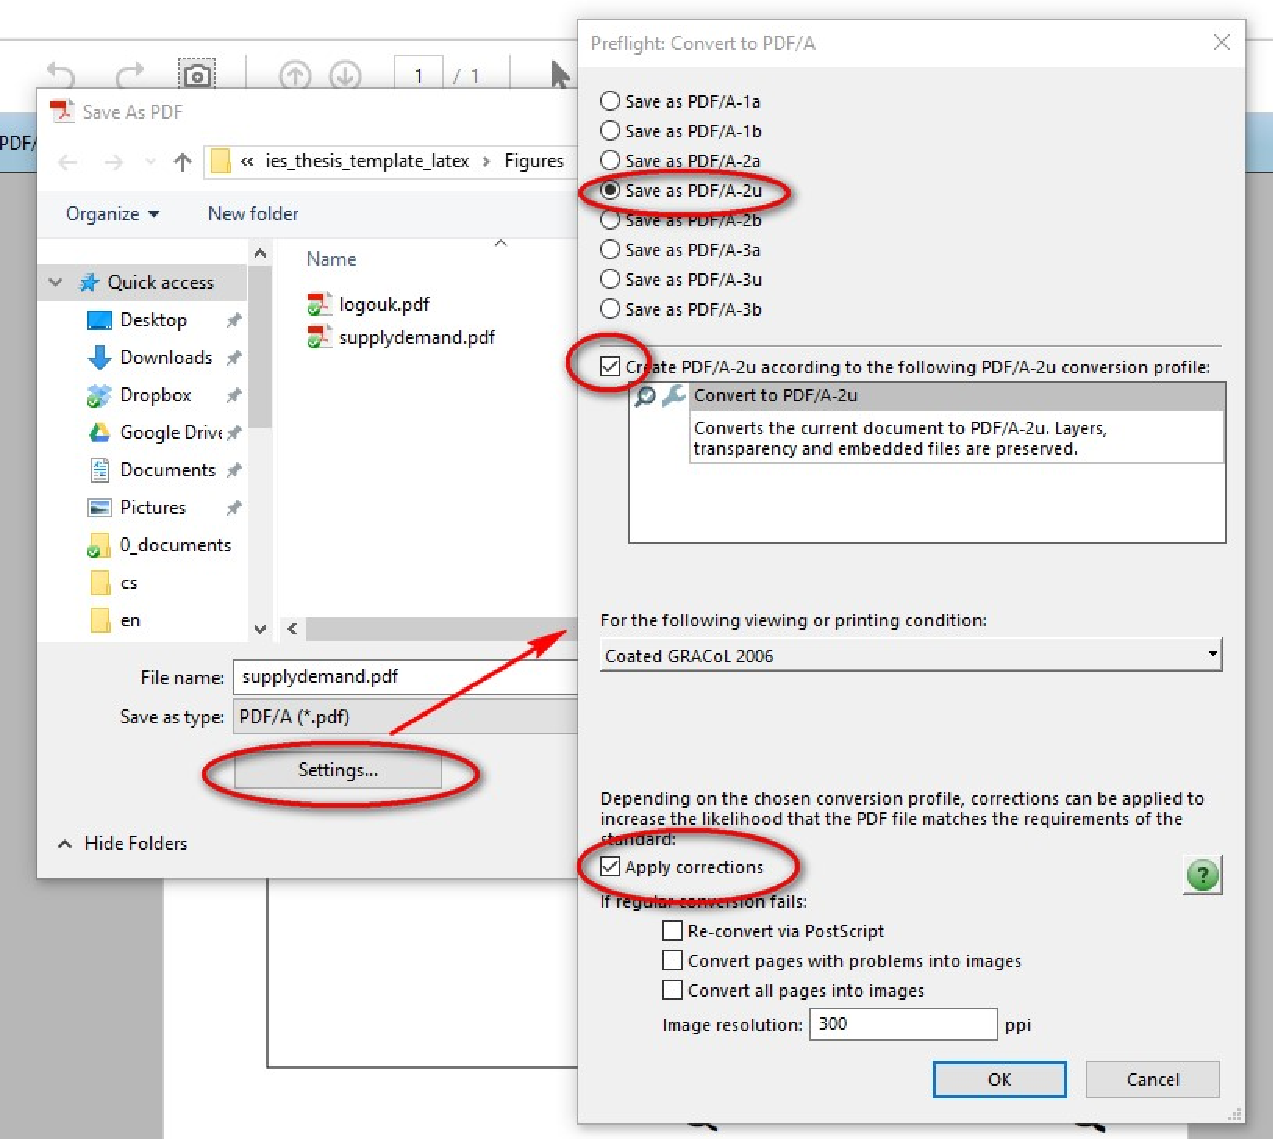
\includegraphics[width=0.6\textwidth]{Figures/conversion2.pdf}
				\label{fig:conversion2}
			\end{figure}
\end{itemize}	


But most of the vector graphics gets distorted to lower quality in Adobe (like pictures in pdfs generated from Stata, unless jpeg is sufficient for you).
You can also use GhostScript, the conversion tool is provided by courtesy of the Faculty of Mathematics and Physics at

\vspace{0.5cm}
\textbf{\href{https://kam.mff.cuni.cz/pdfix/}{https://kam.mff.cuni.cz/pdfix/}}
\vspace{0.5cm}

Text text text text text text.\footnote{Text text text text text text text text text text text text text text text. Text text text text text text text text text text.Text text text text text text.}
Font of Latin phrases should be consistent: Furthermore, there is no \latinfont{ex post} price effect, all things being equal (\latinfont{ceteris paribus}). This is \latinfont{per se} truth.

\begin{figure}[!htbp]
\begin{center}
\caption{Market equilibrium}
\label{fig:supply}
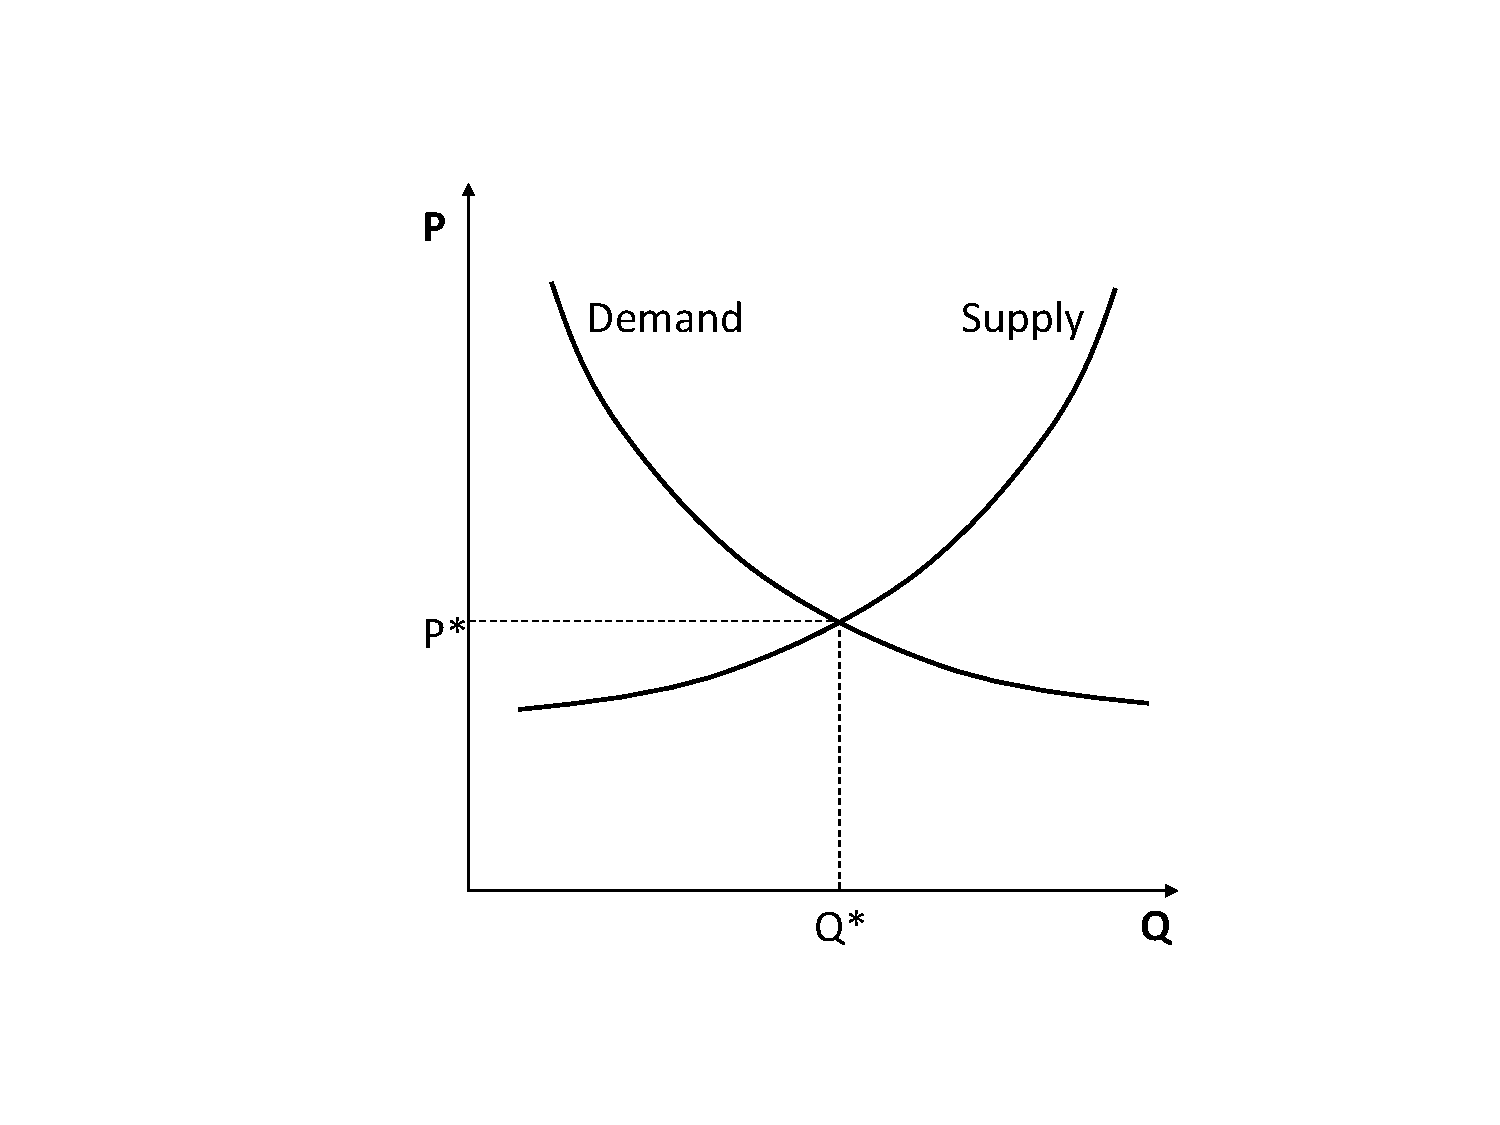
\includegraphics[width=60mm]{Figures/supplydemand}
\end{center}\vspace{-0.5cm}
\begin{source}\cite{Haufler2006}.\end{source}
\end{figure}

Look at the \autoref{fig:supply}. Text text text text text text text text text text.



\section{Tables}

If you use Stata, you might want to check the \texttt{sutex}, \texttt{outtable}, \texttt{outtex}, and \texttt{estout} tools, which help you with exporting Stata tables to \LaTeX{}.

\begin{table}[!htbp]
\begin{center}
	\caption[Calibration table]{Model's predictions}\label{tab:values}
\begin{tabular}{lrrrrrrrrrr}
\toprule
\textit{Case} &        $Y_1$ &        $Y_2$ &  $\tau_1$ &  $\tau_2$ &          $a$ &          $n$\\
\midrule
CR---Slovakia &       10.9 &         10 &       0.24 &       0.19 &          1,000 &       2.16\\

CR---Poland &       13.3 &         12 &       0.24 &       0.19 &          1,000 &       0.38\\

CR---Hungary &       10.4 &          8 &       0.24 &       0.16 &          1,000 &        1.10\\
\bottomrule
\end{tabular}  
\end{center}
\begin{source} If the source is author himself (like a calculation output), this line is redundant.\end{source}
\end{table}

Text text text text text text text text text text text text text text text.


\section{Boxes}
Text text text text text text text text text text text text text text text. Let us make a box:

\begin{figure}[!htbp]
\begin{center}
\caption{Boxy's example}\label{box:values}
\begin{boxeditemize}
	\item Welcome to Boxy paragraph. 
We sincerely hope you will
all enjoy the show.
	\item
Welcome to Boxy paragraph.
We sincerely hope you will
all enjoy the show.
	\item 
Welcome to Boxy paragraph.
We sincerely hope you will
all enjoy the show.
\end{boxeditemize}
\end{center}
\begin{source}\cite{Haaparanta1996}\end{source}
\end{figure}

Text text text text text text text text text text text text text text text.

\section{Theorems, Definitions, \ldots}

\begin{defin}[My original definition]\label{de:definice1}
This is a definition.
\end{defin}

\begin{ass}[My realistic assumption]\label{as:predpoklad1}
This is an assumption.
\end{ass}

\begin{prop}[My clever proposition]\label{pr:veta1}
This is a proposition.
\end{prop}

\begin{lemma}[My useful lemma]\label{le:lemma1}
This is a lemma.
\end{lemma}

\begin{exam}\label{ex:priklad1}
This is an example.
\end{exam}

\begin{proof}
This is a proof.
\end{proof}

\section{Nonumbered Equations}


    \[ U = \underbrace{\int_0^{\infty} \frac{1}{1-\sigma}\left(C^{1-\sigma} -1 \right) e^{-\rho t} \ud t}_\text{meaning of life} \]


\section{Numbered Equations}

\begin{equation}\label{eq:rovnice1}
    U = \int_0^{\infty} \overbrace{ \frac{1}{1-\sigma}\left(C^{1-\sigma} -1 \right)}^\text{instantaneous utility} e^{-\rho t} \ud t
\end{equation}

\section{Matrix Equations}

\begin{equation}\label{eq:rovnice2}
    \mat{A} = \mat{B} + \mat{C}
\end{equation}

\section{Cross-references}

\begin{itemize}
    \item to literature~\citep[pg.~10]{Bjorvatn2006} 	
            or~\citet[pg.~10]{Haufler2006},
    \item to~\autoref{fig:supply},														%or use \autoref
    \item see~\autoref{tab:values},
    \item to~\autoref{rovnice},
    \item to~\defref{de:definice1}, to~\proref{pr:veta1},
            \exaref{ex:priklad1}, 
    \item to equations like this: see~\eqref{eq:rovnice1}.
\end{itemize}

\section{Source codes}

You can input a source code like this:
\begin{matlab}{.9\linewidth}{dgreen}
    omega = 1;
    syms zeta;
    jmn = [1 2*zeta*omega omega^2];
    figure(1);
        for zeta = 1E-5 : 0.2 : 1+1E-12
            G = tf(omega^2,subs([1 2*zeta*omega omega^2]));
            bode(G); hold on;
        end
    legend('\zeta = 0','\zeta = 0,2','\zeta = 0,4','\zeta = 0,6',');
\end{matlab}
Should you prefer a different font size, redefine file \texttt{Styles/Mystyle.sty}.



\section{Paragraphs}

Usually you should not use the first person singular (I) in your text, write we instead.
As a general recommendation, use the first person sparsely, sometimes it can be replaced by a phrase like ``This work presents \ldots.''

Text text text text text text \citep{Haufler2006}. Let us make two paragraphs:

\paragraph{Proin} Text text text text text text text text text text text text text text text. Text text text text text text. And a subparagraph:
\subparagraph{Velit} Text text text text text text text text text text text text text text text.






